\section{Flots et coupes}
\subsection{Flots et coupes}
\index{flot}
\index{capacité}
\begin{mydef}
  Soit un graphe dirigé, dont les noeuds sont partitionnés en sources, puits et noeuds intermédiaires, et dont chaque arête $a$ porte un nombre réel $c(a)$ nommé \emph{capacité}.\\
  Un \emph{flot} est la donnée d'un nombre réel $f(a)$ sur chaque arête, tel que $0 \leq f(a) \leq c(a)$ et que le flot net sortant de chaque noeud intermédiaire soit nul.
\end{mydef}

\index{flot!flot net sortant}
\index{flot!valeur du flot}
\index{flot!flot maximum}
\begin{mydef}
  Le \emph{flot net sortant d'un noeud} $u$ est défini comme
  $\sum_{\text{arêtes }a\text{ d'origine }u} f(a) − \sum_{\text{arêtes }b\text{ de destination }u} f(b)$.
  Le \emph{flot net sortant d'un ensemble} $U$ de noeuds est la somme des flots nets sortant des noeuds de $U$.\\
  La \emph{valeur du flot} est le flot net sortant des noeuds sources.\\
  On désire trouver le \emph{flot maximum}, c'est-à-dire le flot de valeur maximale.
\end{mydef}

\index{coupe}
\index{coupe!coupe minimum}
\begin{mydef}
  Une \emph{coupe} est un ensemble d'arêtes tel qu'il n'ait plus aucun chemin d'un noeud source vers un noeud puits quand on retire cet ensemble du graphe.\\
  On désire trouver une \emph{coupe minimum}, c'est-à-dire une coupe dont la capacité (i.e., la somme des capacités de ses arêtes) est minimale.
\end{mydef}

\begin{center}
  \begin{tikzpicture}
    \node[vertex] at (0, 0) (s) {\tiny $s$};
    \node[vertex] at (2, 1) (a) {\tiny $a$};
    \node[vertex] at (2, -1) (b) {\tiny $b$};
    \node[vertex] at (4, 1) (c) {\tiny $c$};
    \node[vertex] at (4, -1) (d) {\tiny $d$};
    \node[vertex] at (6, 0) (t) {\tiny $t$};
    \draw[->] (s) edge node[anchor = south] {\tiny $0 / 3$} (a);
    \draw[->] (s) edge node[anchor = north] {\tiny $0 / 2$} (b);
    \draw[->] (a) edge node[anchor = south] {\tiny $0 / 2$} (c);
    \draw[->] (a) edge node[anchor = south] {\tiny $0 / 3$} (d);
    \draw[->] (b) edge node[anchor = north] {\tiny $0 / 2$} (d);
    \draw[->] (c) edge node[anchor = south] {\tiny $0 / 2$} (t);
    \draw[->] (d) edge node[anchor = north] {\tiny $0 / 2$} (t);
  \end{tikzpicture}
\end{center}

\begin{center}
  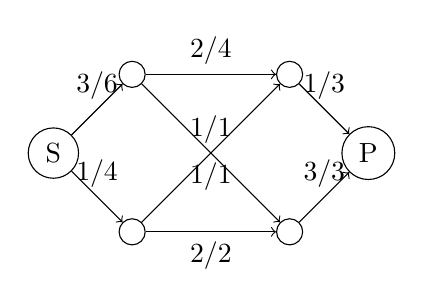
\begin{tikzpicture}
    \node[draw, circle] at (-2,0) (S) {S};
    \node[draw, circle] at (-1,1) (A) {};
    \node[draw, circle] at (-1,-1) (B) {};
    \node[draw, circle] at (1,1) (C) {};
    \node[draw, circle] at (1,-1) (D) {};
    \node[draw, circle] at (2,0) (P) {P};

    \draw[->] (S) edge node[anchor = south] {$3/6$} (A);
    \draw[->] (S) edge node[anchor = south] {$1/4$} (B);
    \draw[->] (A) edge node[anchor = south] {$2/4$} (C);
    \draw[->] (A) edge node[anchor = south] {$1/1$} (D);
    \draw[->] (B) edge node[anchor = north] {$1/1$} (C);
    \draw[->] (B) edge node[anchor = north] {$2/2$} (D);
    \draw[->] (C) edge node[anchor = south] {$1/3$} (P);
    \draw[->] (D) edge node[anchor = south] {$3/3$} (P);
  \end{tikzpicture}
\end{center}

\paragraph{Observation}
Se donner une coupe, on se donne un ensemble $S$ de noeuds atteignables à partir des sources,
c'est la même chose.
Lorsqu'on a une coupe, $S$ est la composante connexe comprenant les sources lorsqu'on enlève la coupe.
Lorsqu'on a $S$, la coupe est l'ensemble des arêtes reliant un noeud de $S$ et de $\bar{S}$.

\begin{mylem}
  Pour un flot donné, toutes les coupes ont le même flot net, qui est la valeur du flot.
  \begin{proof}
    Flot net de la coupe = Flot net(sources) + Flot net (s$\setminus$sources)
    =$f(S \to \bar{S}) - f(\bar{S} \to S)$
    taille de la coupe = capacité totale de la coupe
    \begin{center}
      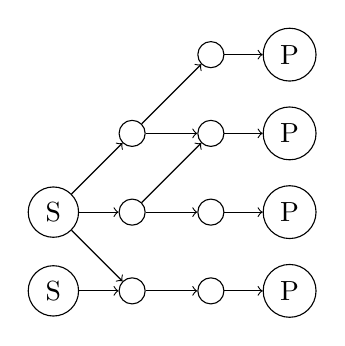
\begin{tikzpicture}
        \node[draw, circle] at (-2,0) (S1) {S};
        \node[draw, circle] at (-2,-1) (S2) {S};
        \node[draw, circle] at (-1,1) (A1) {};
        \node[draw, circle] at (-1,0) (A2) {};
        \node[draw, circle] at (-1,-1) (A3) {};
        \node[draw, circle] at (0,2) (B1) {};
        \node[draw, circle] at (0,1) (B2) {};
        \node[draw, circle] at (0,0) (B3) {};
        \node[draw, circle] at (0,-1) (B4) {};
        \node[draw, circle] at (1,2) (P1) {P};
        \node[draw, circle] at (1,1) (P2) {P};
        \node[draw, circle] at (1,0) (P3) {P};
        \node[draw, circle] at (1,-1) (P4) {P};

        \draw[->] (S1) edge (A1);
        \draw[->] (S1) edge (A2);
        \draw[->] (S1) edge (A3);
        \draw[->] (S2) edge (A3);
        \draw[->] (A1) edge (B1);
        \draw[->] (A1) edge (B2);
        \draw[->] (A2) edge (B2);
        \draw[->] (A2) edge (B3);
        \draw[->] (A3) edge (B4);
        \draw[->] (B1) edge (P1);
        \draw[->] (B2) edge (P2);
        \draw[->] (B3) edge (P3);
        \draw[->] (B4) edge (P4);
      \end{tikzpicture}
    \end{center}
  \end{proof}
\end{mylem}

\begin{mylem}
  Pour tout flot $f$ et toute coupe $S \to \bar{S}$, valeur($f$) $\leq$ capacité($S \to \bar{S}$). L'égalité a lieu si et seulement si toutes les arêtes $a$ de la coupe $S \to \bar{S}$ sont $f$-saturées (i.e., $f(a) = c(a)$) et toutes les arêtes $b$ de $\bar{S} \to S$ sont $f$-nulles (i.e., $f(b) = 0$).

  \begin{proof}
    \begin{align*}
      \mathrm{valeur}(f) & = \text{flot sur la coupe}\\
             & = \sum f_{\mathrm{net}}(S \to \bar{S})\\
             & = \sum_{i \in S \atop {j \in \bar{S} \atop ij \in E}} f_{ij} - \sum_{i \in S \atop {j \in \bar{S} \atop ji \in E}} f_{ij}\\
             & \leq \sum_{i \in S \atop {j \in \bar{S} \atop ij \in E}} f_{ij}\\
             & \leq \sum_{i \in S \atop {j \in \bar{S} \atop ij \in E}} c_{ij}\\
             & = \text{Coupe}(S \to \bar{S}).
    \end{align*}
    Avec égalité si et seulement si $\sum_{i \in S\atop {j \in \bar{S}\atop ji \in E}} f_{ij} = 0$ et
    $\sum_{i \in S\atop {j \in \bar{S}\atop ij \in E}} f_{ij} = \sum_{i \in S\atop {j \in \bar{S}\atop ij \in E}} c_{ij}$
    c'est à dire que toutes les arêtes qui lient un noeud de $S$ à un noeud de $\bar{S}$ sont saturées
    et que les arêtes qui lient un noeud de $\bar{S}$ à un noeud de $S$ ont un flot nul.
  \end{proof}
\end{mylem}

\begin{mycorr}
  Si un flot et une coupe sont tels que valeur(flot) = capacité(coupe), alors ce flot est maximum et cette coupe minimum.
  \begin{proof}
    On vient de voir que dans le cas d'égalité, les arêtes étaient saturées et il n'y a aucun flot qui va de $\bar{S}$ à $S$
    Et donc ne peut plus faire passer de flot de $S$ à $\bar{S}$ ni par des arêtes directes (elles sont saturées),
    ni par des ``back edges'' (elles sont nulles car il n'y a pas de flot de $\bar{S}$ à $S$).

    Le fait que le flot est maximum et que la coupe est minimum est en fait simplement montré par la dualité.
    On sait que pour toute coupe $S\to\bar{S}$ et flot $f$, $\text{Coupe}(S\to\bar{S}) \geq \mathrm{valeur}(f)$.
    Dès lors, pour toute coupe $\text{Coupe}(S \to \bar{S}) \geq f_\mathrm{max}$ et pour tout flot,
    $\text{Coupe}_\mathrm{min} \geq \mathrm{valeur}(f)$ et en particulier $\text{Coupe}_\mathrm{min} \geq f_\mathrm{max}$.
    On a donc
    \[ \text{Coupe}(S \to \bar{S}) \geq \text{Coupe}_\mathrm{min} \geq f_\mathrm{max} \geq \mathrm{valeur}(f) \]
    d'où $\text{Coupe}(S \to \bar{S}) = \text{Coupe}_\mathrm{min}$ et
    $f_\mathrm{max} = \mathrm{valeur}(f)$ en cas d'égalité
    $\text{Coupe}(S \to \bar{S}) = \mathrm{valeur}(f)$.
  \end{proof}
\end{mycorr}

\index{chemin!chemin $f$-saturé}
\index{chemin!chemin $f$-augmentant}
\begin{mydef}
  Etant donné un flot $f$, à tout chemin $P$ dans le graphe non-dirigé sous-jacent associons la quantité $i(P) = min_{a \in P} i(a)$, où $i(a) = c(a) − f(a)$ pour les arêtes $a$ prises par $P$ dans le sens direct, et $i(a) = f (a)$ pour les arêtes a prises dans le sens inverse.\\
  Un chemin $P$ est \emph{$f$-saturé} si $i(P) = 0$. Il est \emph{$f$-augmentant} s'il est non saturé, part d'un noeud source et arrive à un noeud puits.
\end{mydef}

\begin{mytheo}
  Un flot est maximum si et seulement s'il ne contient pas de chemin $f$-augmentant.
  \begin{proof}
     Preuve \addTODO
  \end{proof}
\end{mytheo}

\begin{mytheo}
  La valeur du flot maximum et la capacité de la coupe minimum sont toujours égales.
  \begin{proof}
     Preuve \addTODO
  \end{proof}
\end{mytheo}

\subsection{L'algorithme de Ford-Fulkerson}
\index{algorithme!algorithme de Ford-Fulkerson}
\begin{myalgo}[Algorithme de Ford-Fulkerson]
  Algorithme \addTODO
\end{myalgo}

\begin{myexem}
  Exemple \addTODO
\end{myexem}

\begin{mylem}
  Dans tout graphe dirigé avec un noeud source $u$ et un noeud puits $v$ et chaque arête de capacité un, le nombre maximum de chemins dirigés de u vers v disjoints deux à deux par les arêtes est la valeur du flot maximum.
  \begin{proof}
     Preuve \addTODO
  \end{proof}
\end{mylem}

\begin{mytheo}
  Un graphe (non-dirigé) est $k$-arête-connexe si et seulement si entre chaque paire de noeuds il y a au moins $k$ chemins disjoints deux à deux par les arêtes.
  \begin{proof}
     Preuve \addTODO
  \end{proof}
\end{mytheo}

\begin{mytheo} [Menger]
  Un graphe (non-dirigé) est $k$-connexe si et seulement si entre chaque paire de noeuds il y a au moins $k$ chemins disjoints deux à deux par les noeuds.
  \begin{proof}
     Preuve \addTODO
  \end{proof}
\end{mytheo}
